\documentclass{beamer}
\usepackage{luatexja} 
\usepackage[ipaex]{luatexja-preset} 
\renewcommand{\kanjifamilydefault}{\gtdefault}

\usepackage{bm} %bold → \mathbf{}
\usepackage{mathtools} 
\usepackage{amsmath} 
\usepackage{amsthm}
\usepackage{setspace}
\usepackage{comment}
\usepackage{url}

\newtheorem{thm}{Theorem}[section] 
\newtheorem{lem}[thm]{Lemma} 
\newtheorem{prop}[thm]{Proposition} 
\newtheorem{assumption}[thm]{Assumption} 
\usetheme{PaloAlto} 
\usecolortheme{dove}
\setbeamertemplate{navigation symbols}{} 

\DeclareMathOperator*{\argmax}{arg\,\max}
\DeclareMathOperator*{\argmin}{arg\,\min}
\renewcommand{\baselinestretch}{0.95}
% cmd / : comment out
%\newcommand{\relmiddle}[1]{\mathrel{}\middle#1\mathrel{}}% resized \mid → relmiddle |

\title{Heterogeneous Impacts of Informal Caregiving on Labor Market Outcomes:} 
\subtitle{Research Proposal}
\author{M1 Inoue Jin}
\institute{Hitotsubashi University} 


\begin{document}

\begin{frame}
    \titlepage
\end{frame}

\begin{frame}{Outline}
    \tableofcontents
\end{frame}

\section{Introduction}

    \subsection{Why does informal caregiving matter?}
        \begin{frame}\frametitle{Why does informal caregiving matter?}
            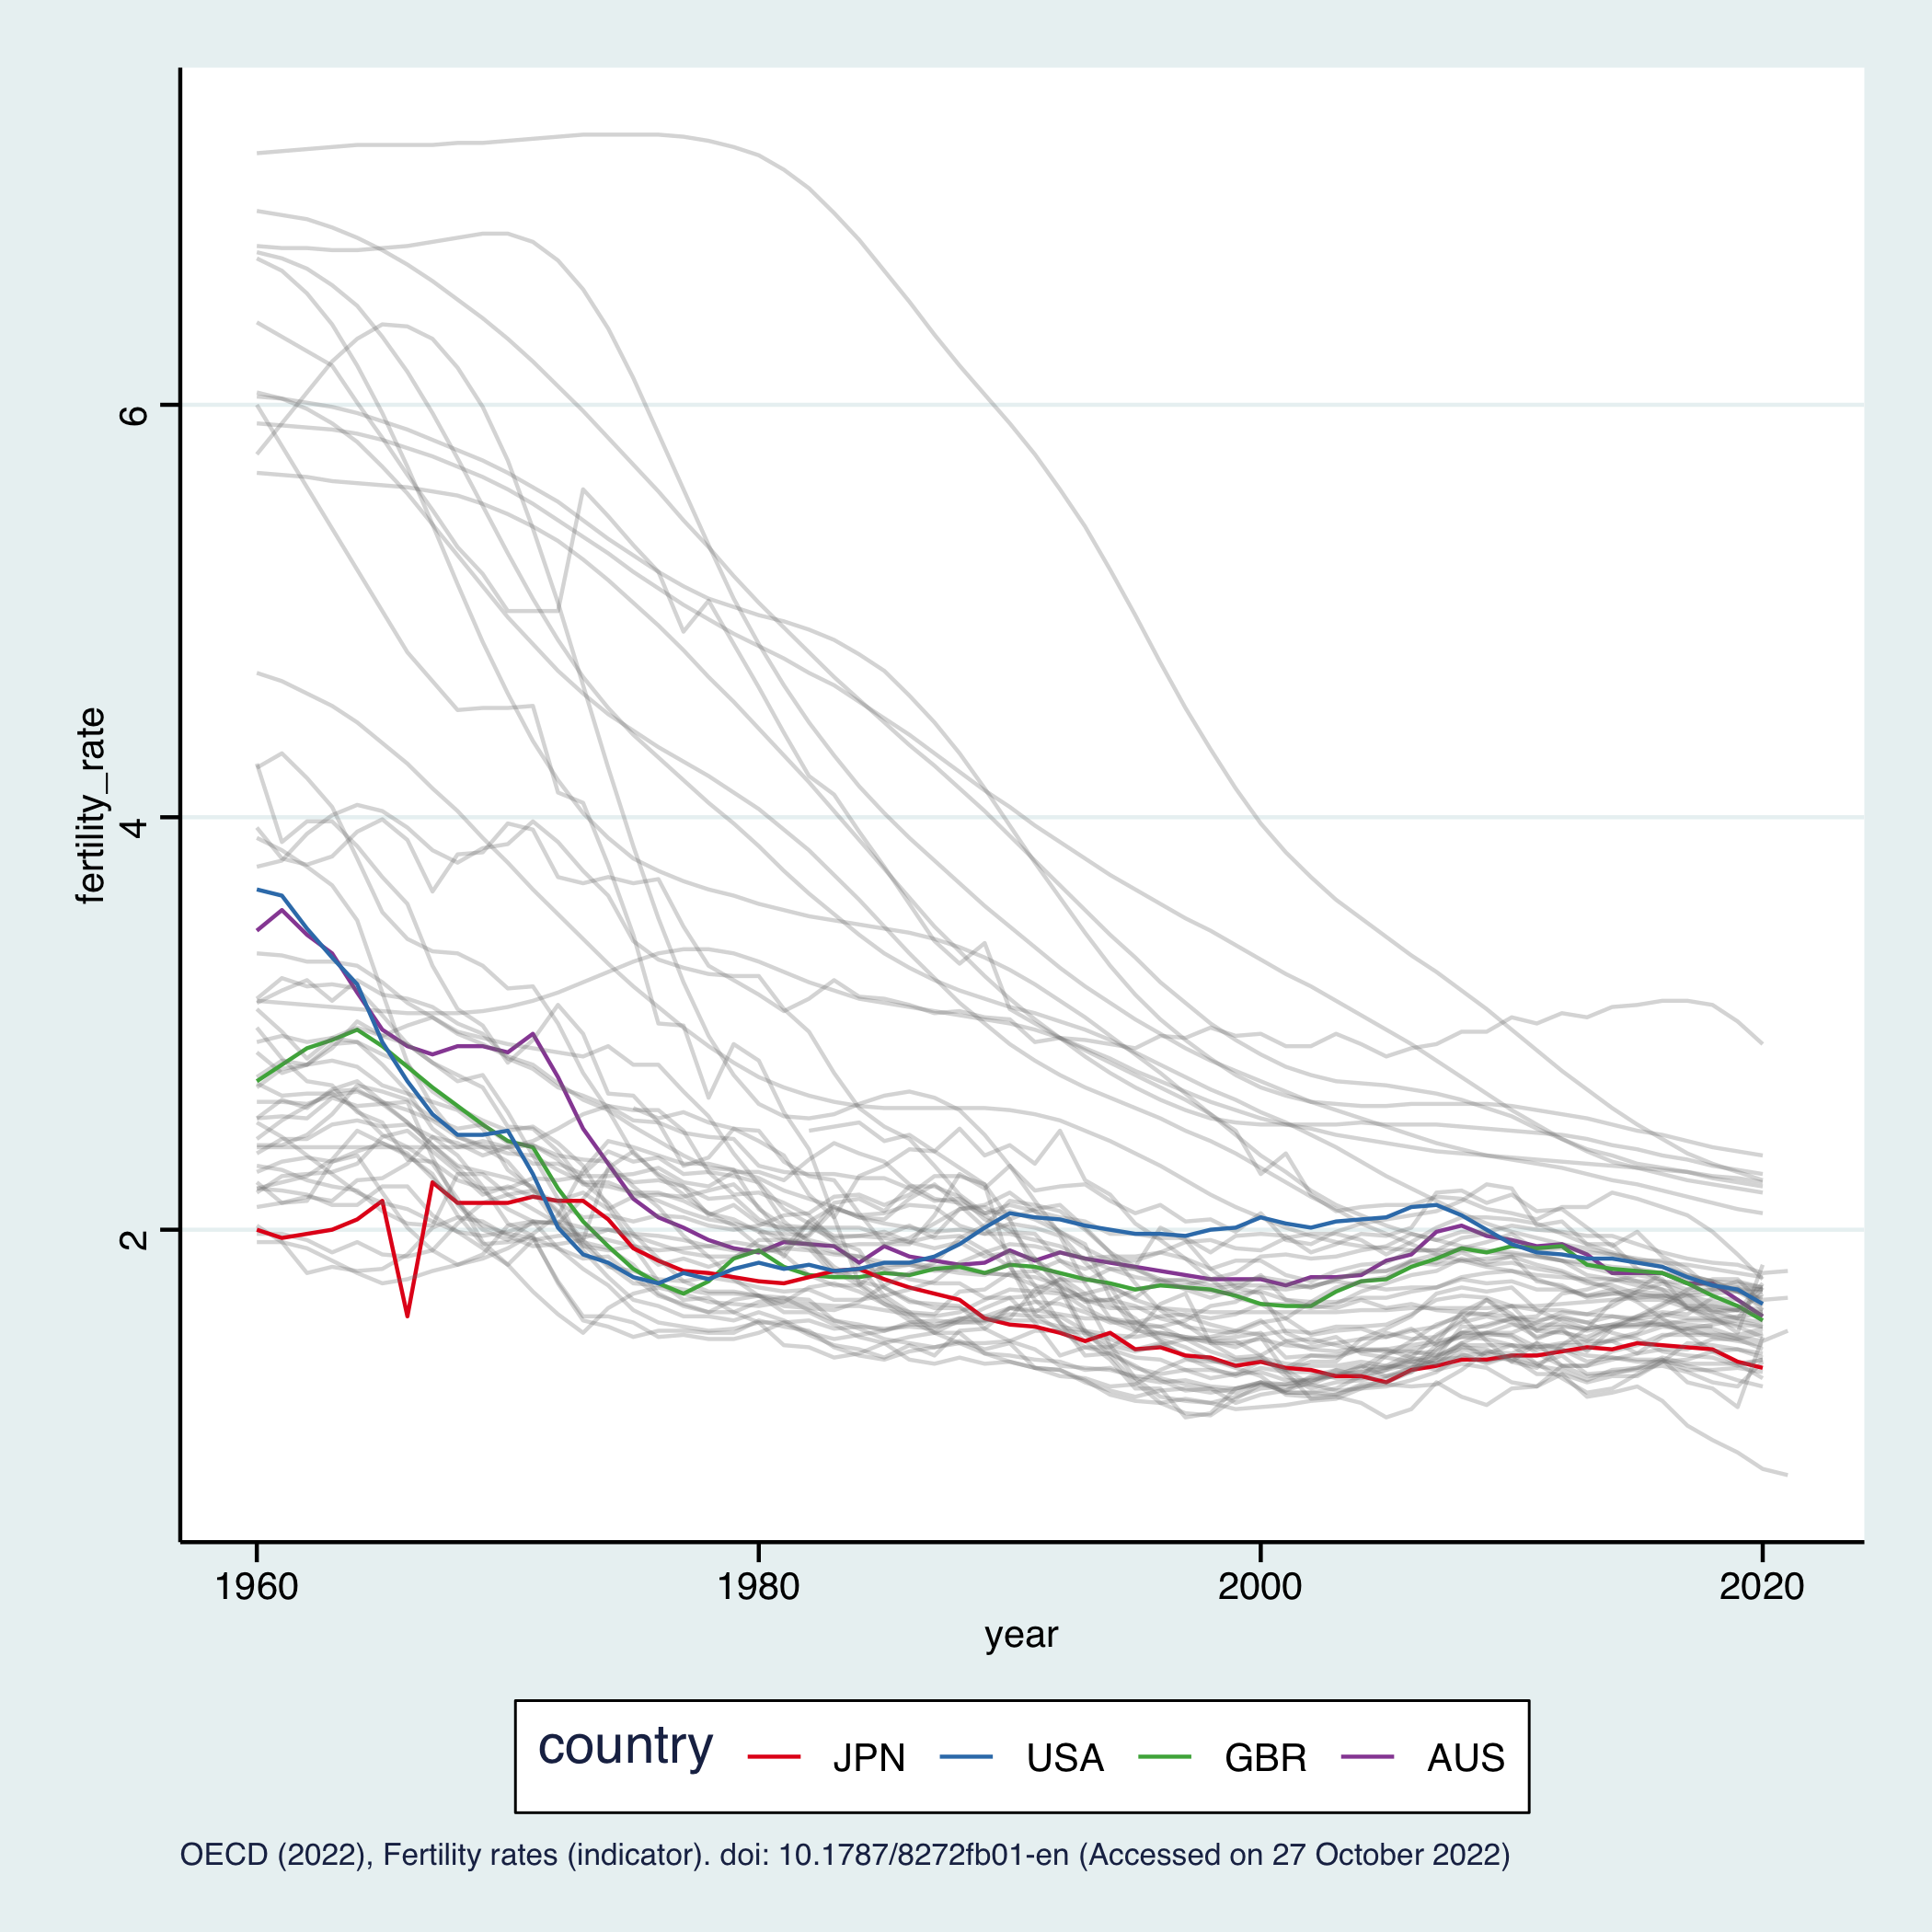
\includegraphics[height = 5cm]{OECD_fertility_rates.png}
            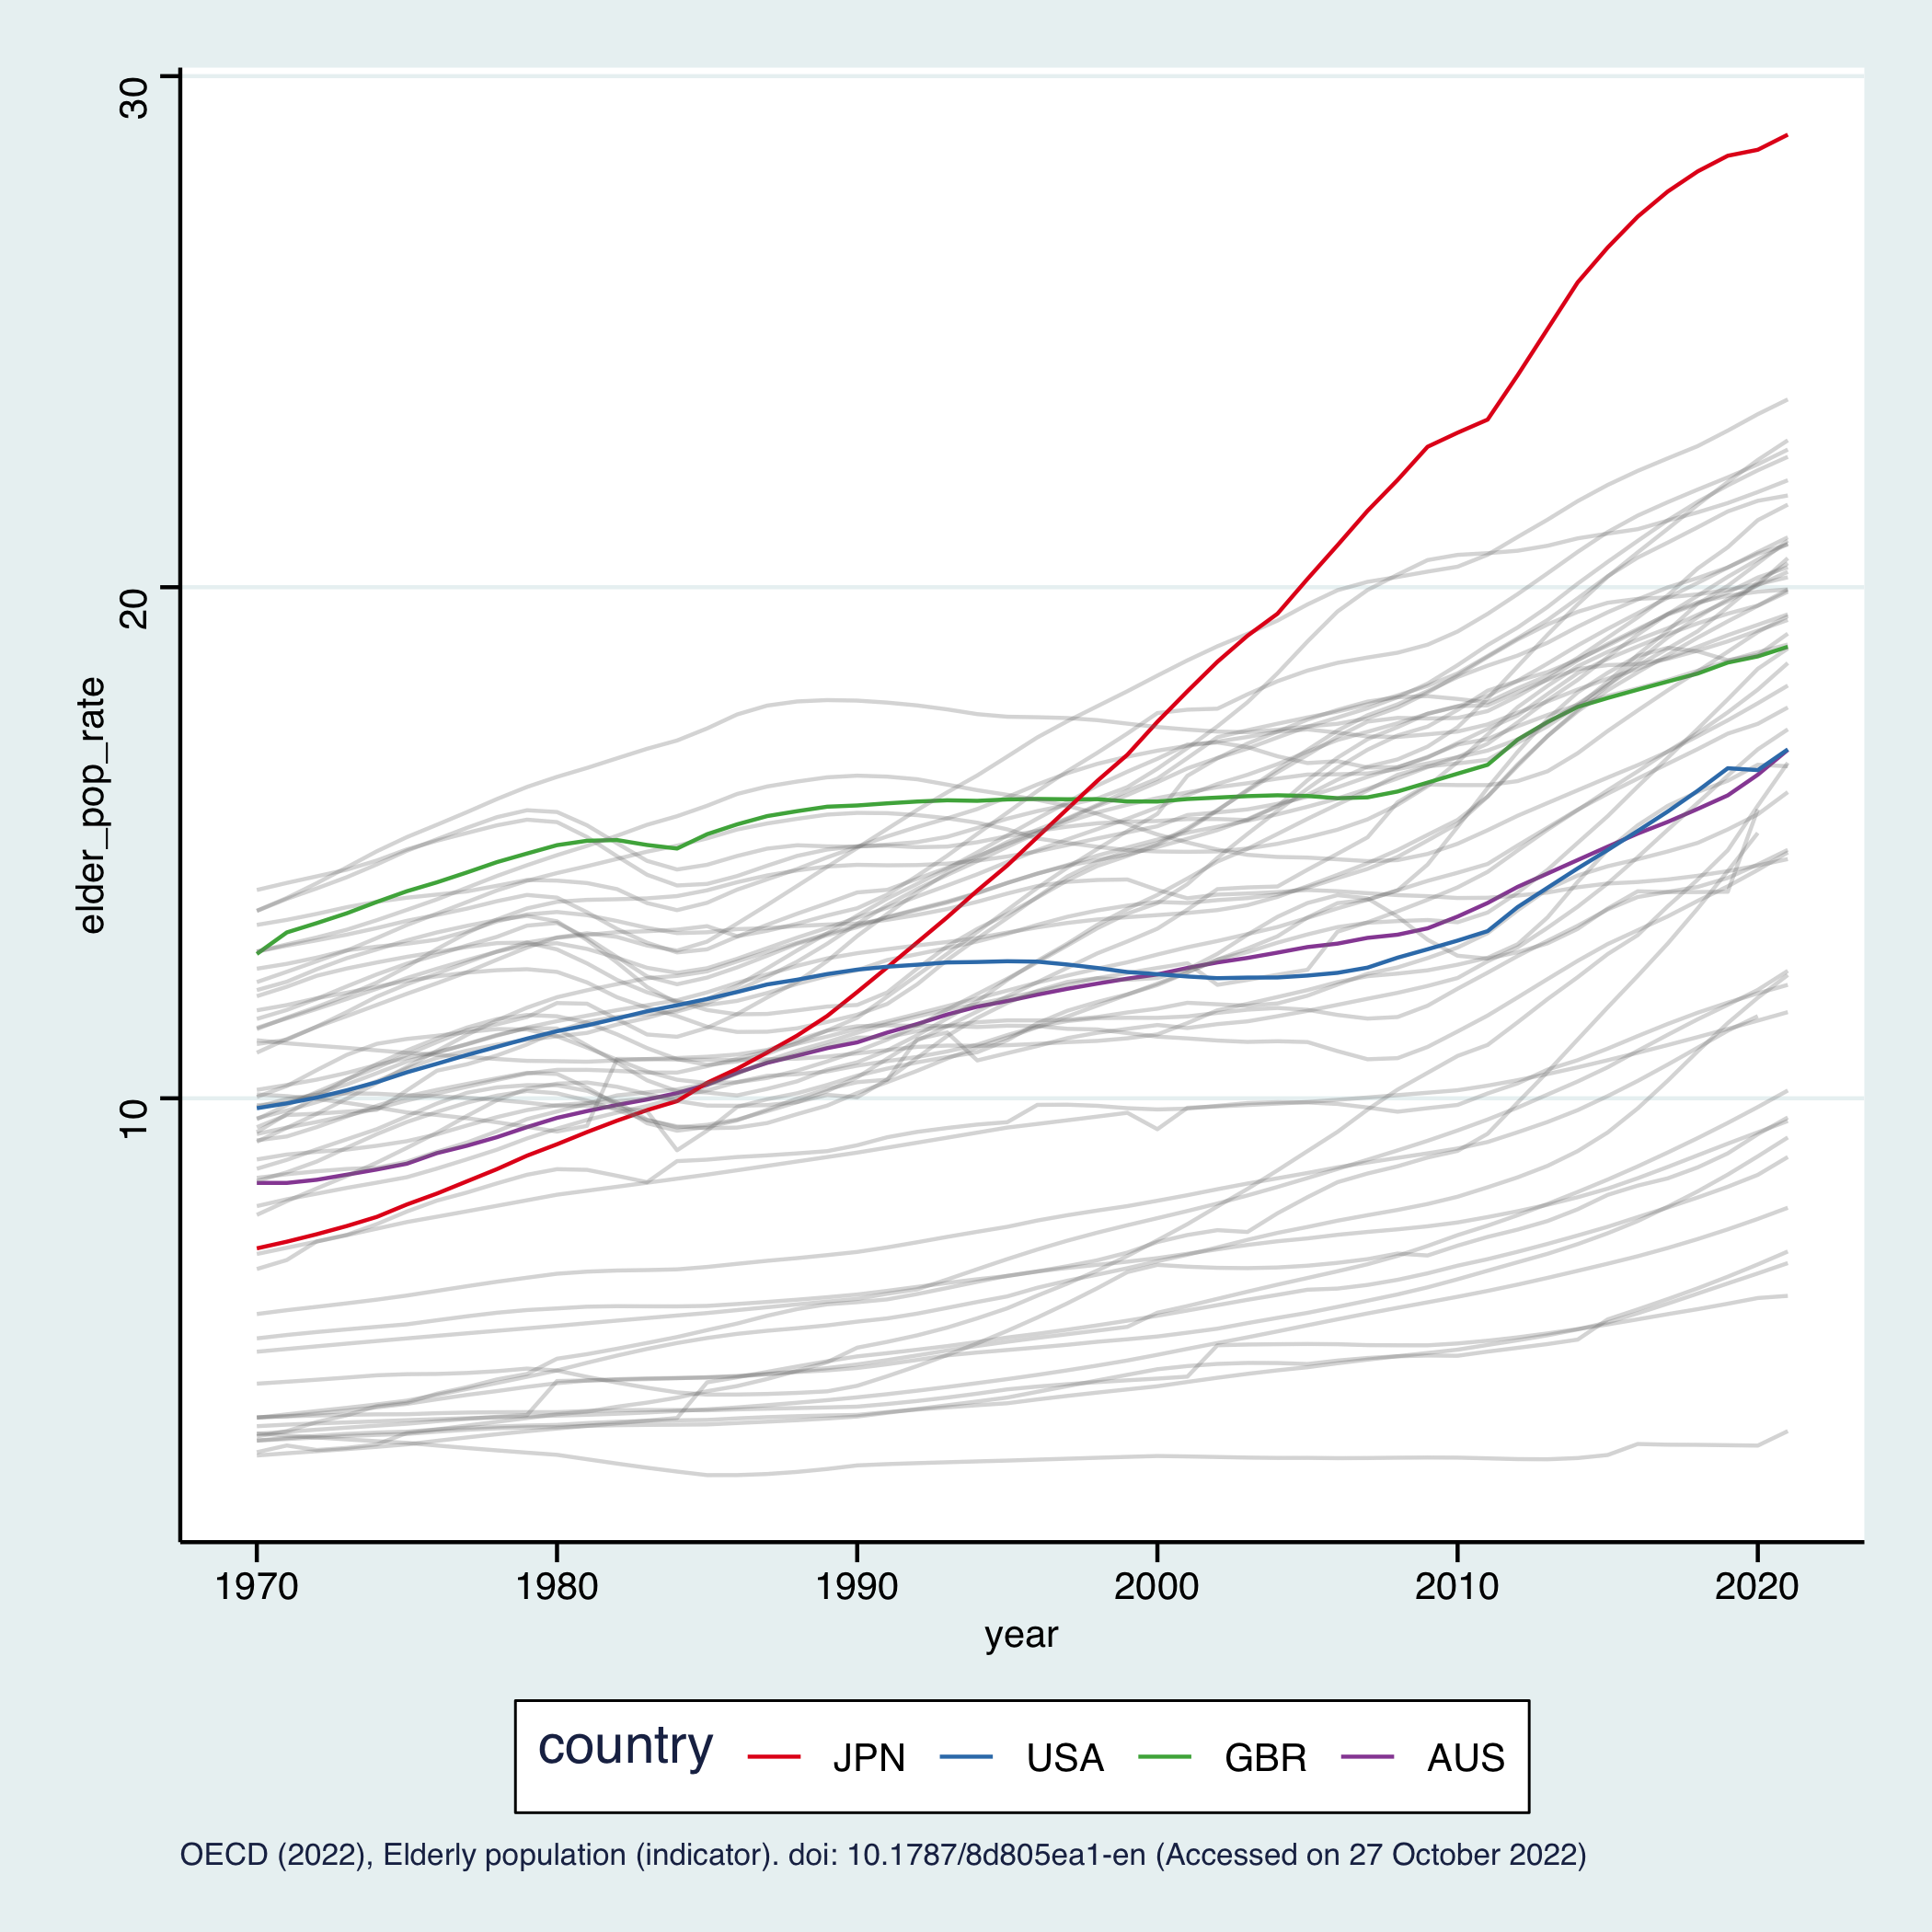
\includegraphics[height = 5cm]{OECD_Elderly_pop_rate.png}
            \begin{itemize}
                \item Most of developed countries are faced with the decline of fertility rates and experiencing aging society.
                \item These trends predict that the supply of labor markets will decrease in the long run while the demand for caregiving will continue to increase. 
            \end{itemize}
        \end{frame}
        \begin{frame}\frametitle{Why does informal caregiving matter?}
            \begin{itemize}
                \item Care-givers face a trade-off between hours of work, leisure and time for care-giving.
                \item Intuitively, there seems to be a negative relationship between care-giving and one's employment and hours of work. But empirically, it's not obvious whether informal caregiving has negative effects on one's employment, hours of work, and some labor market outcomes.  
            \end{itemize}
        \end{frame}

    \subsection{Literature review}
        \begin{frame}\frametitle{Literature review:}
            \begin{itemize}
                \item Almost all the literature show the negative estimates except for Wolf and Soldo(1994).
                \item Many of the previous literature used panel data and found that negative fixed effects estimates of informal care on LFP is smaller in its size than cross-section OLS estimates.(Heitmueller, 2007;Bolin et al., 2008;Leigh, 2010;Van Houtven et al., 2013; Oshio and Usui, 2018)
            \end{itemize}
        \end{frame}
        \begin{frame}\frametitle{Literature review:endogeneity}
            \begin{itemize}
                \item There is a concern for an endogeneity of the provision of informal caregiving. The provision of informal caregiving as a treatment variable($D_{it}$) is assumed to be correlated with the potential employment status as outcomes($Y_{it}(D_{it})$)
                \item For example, there are caregivers who were unemployed before the needs for caring arises. Also, individuals who has less attachment to work in their household is likely to be informal-caregiver.
            \end{itemize}
        \end{frame}
        \begin{frame}\frametitle{Literature review:endogeneity}
            \begin{itemize}
                \item Previous literature deal with the endogeneity problem with instrumental variables.
                \item Instruments are :
                \begin{itemize}
                    \item the number of disabled people in the household and the age of friends of the respondent(Heitmueller, 2007).
                    \item Mother/father have bad health, lives far away, deceased, their age and the number of siblings(Bolin et al., 2008)
                    \item Separate indicators for the mother or mother-in-law being ill and separate indicators for the mother or mother-in-law becoming widowed since the last survey wave...etc(Van Houtven et al., 2013)
                \end{itemize}
            \end{itemize}
        \end{frame}
        \begin{frame}\frametitle{Literature review:endogeneity}
            \begin{itemize}
                \item However, in those literature, they could not reject the null hypothesis of the exogeneity of treatment variable.(Heitmueller, 2007;Bolin et al., 2008;Van Houtven et al., 2013; Oshio and Usui, 2018)
                \item Most of the endogeneity may be explained by the correlation between time-invariant individual heterogeneity and the treatment variable.
            \end{itemize}
        \end{frame}

    \subsection{Summary}
        \begin{frame}\frametitle{Summary}
            \begin{itemize}
                \item Most of the previous literature support the negative effects of informal caregiving on labor force pariticipation.
                \item They cannot reject the null hypothesis of the exogeneity of the treatment.
                \item By using FE estimator, the negative estimates get smaller than that of OLS estimator.
            \end{itemize}
        \end{frame}

\section{Expected Contribution}
    
        % \subsection{Key point of expected contribution}
        %     \begin{frame}\frametitle{Expected contributions:}
        %         \begin{itemize}
        %             \item By applying a decomposition of FE estimator(de Chaisemartin and D'Haultfœuille, 2020), I suggest negative estimates acquired in preivious literature may underestimate the absolute size of the effects.
        %             \item There may be some heterogeneity of effects in terms of the various lengths of the treatment.
        %         \end{itemize}
        %     \end{frame}

        % \subsection{Applying a decomposition of FE estimator}
        %     \begin{frame}\frametitle{Applying a decomposition of FE estimator}
        %         \begin{block}{Theorem1:de Chaisemartin and D'Haultfœuille(2020)}
        %             Suppose that some assumptions hold. Then,
        %             \begin{equation*}
        %                 \beta_{fe} = \mathbb{E}\left[\sum_{(g,t):D_{g,t}=1}\frac{N_{g,t}}{N_{1}}w_{g,t}\Delta_{g,t}\right]
        %             \end{equation*}
        %         \end{block}
        %         \begin{itemize}
        %             \item Due to the weights $w_{g,t}$ attached, $\beta_{fe}$ does not recover the true effect. 
        %             \item The point is that, sometimes, the weights may be negative.
        %         \end{itemize}
        %     \end{frame}
        %     \begin{frame}\frametitle{Applying a decomposition of FE estimator}
        %         From the section of literature review, the effect of informal caregiving is assumed to be negative($\Delta_{g,t} < 0$). Then, if some of the weights are negative, 
        %         \begin{align*}
        %             \beta_{fe} &= \mathbb{E}\left[\sum_{w_{g,t}>0}\frac{N_{g,t}}{N_{1}}w_{g,t}\Delta_{g,t} + \sum_{w_{g,t}<0}\frac{N_{g,t}}{N_{1}}w_{g,t}\Delta_{g,t}\right]
        %             \\&= \text{negative effects} + \text{positive bias} 
        %             \\&> \text{"true" negative effects}
        %         \end{align*}
        %         \begin{itemize}
        %             \item Negative and small effects obtained by FE estimator may be contaminated by this upward bias.
        %             \item At least, it is possible to avoid this negative weights issue by using de Chaisemartin and D'Haultfœuille(2020)'s alternative DiD estimator for ATT.
        %         \end{itemize}
        %     \end{frame}
    
    \subsection{Focusing on time-heterogeneous treatment effects}
        \begin{frame}\frametitle{Focusing on time-heterogeneous treatment effects}
            \begin{itemize}
                \item About the reason why the negative estimates are small, Leigh(2010) points out that there is a posibbility that the effects of caregiving on labor market outcomes might take several years to manifest itself.
                \item Acoording to a national representative survey (Caregiving in the U.S., 2020) in the U.S.,
                    \begin{itemize}
                        \item 3 in 10 have stopped saving(28\%)
                        \item 1 in 4 have taken on more debt(23\%)
                        \item Both of which could have longer-term aftereffects on caregiver's financial security into the future, especially if the caregiving lasts a long time.
                    \end{itemize}
            \end{itemize}
        \end{frame}
        \begin{frame}\frametitle{Focusing on time-heterogeneous treatment effects}
            \begin{center}
            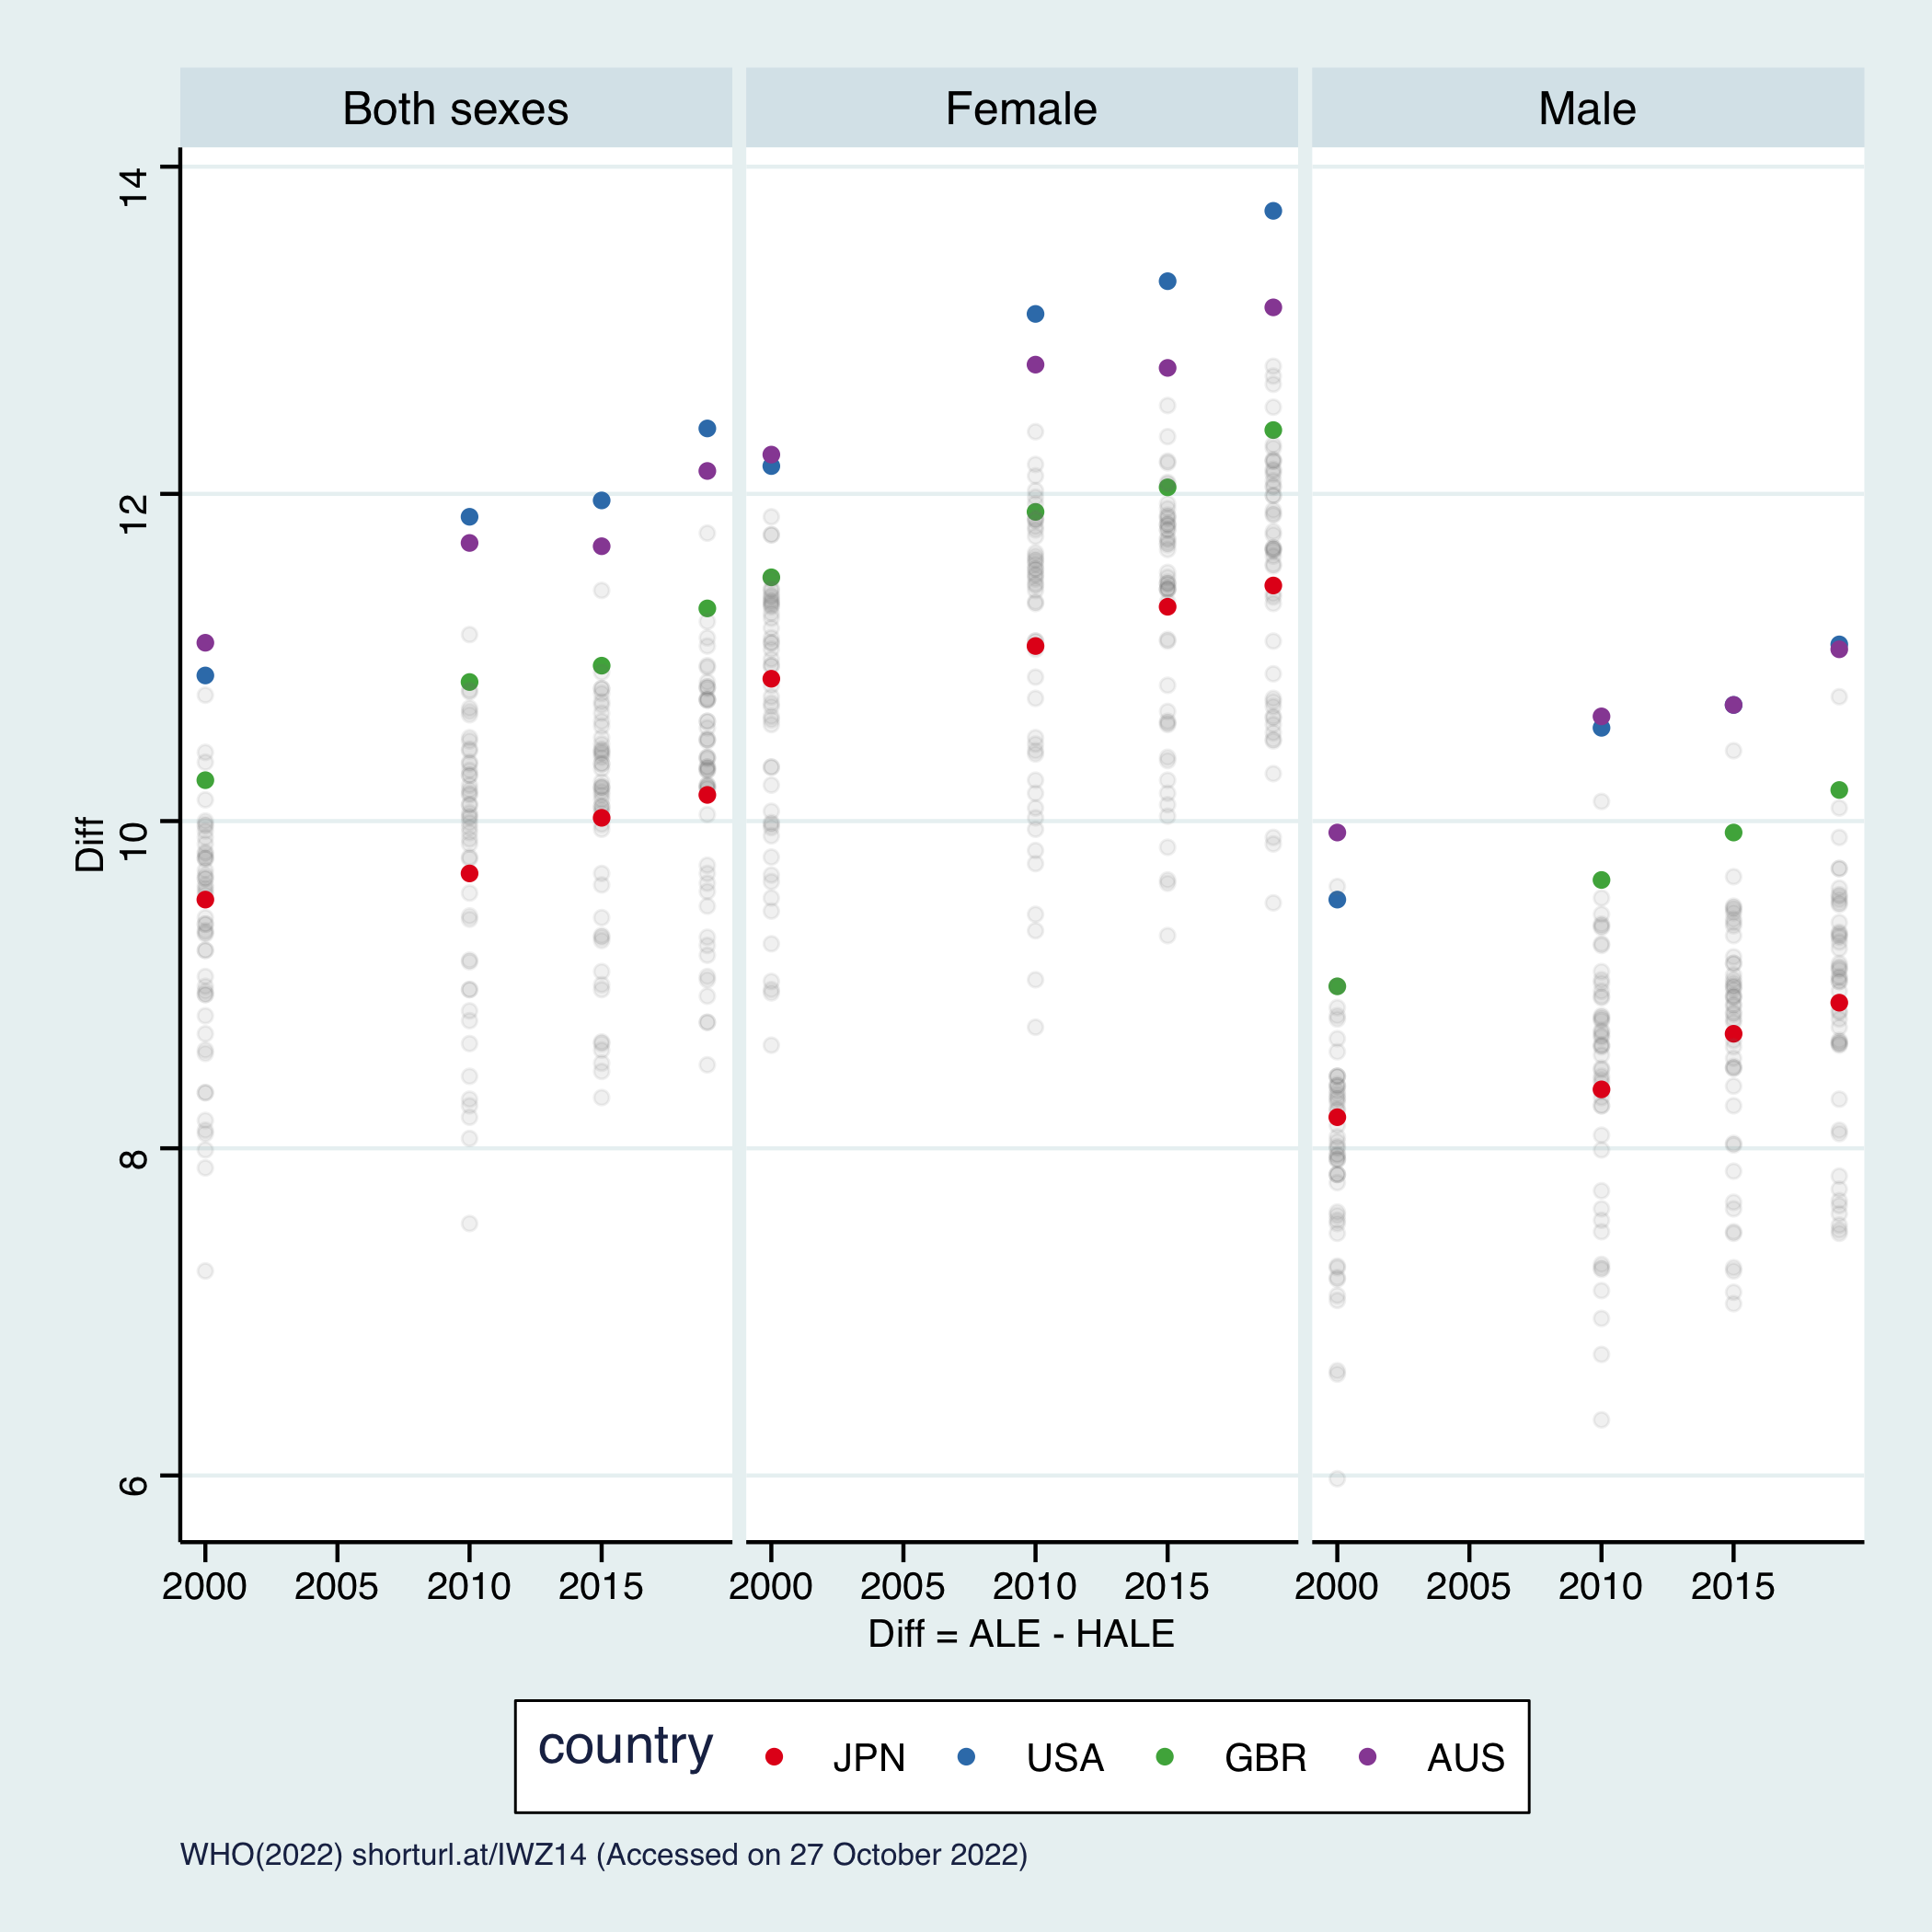
\includegraphics[height = 4.5cm]{WHO_diff_expectancy.png}
            \end{center}
            \footnotesize
            \begin{itemize}
                \item ALE = (Average) Life Expectancy
                \item HALE = Healthy Life Expectancy
                \item The difference of ALE and HALE is the expected length of years one needs care in some way.
                \item This figure implies that the expected length of informal caregiving will be longer in the future.
            \end{itemize}
            \normalsize
        \end{frame}
        \begin{frame}\frametitle{Focusing on time-heterogeneous treatment effects}
            A conventional model for estimating dynamic treatment effects is what we call, "event-study design".
            \begin{block}{event-study design:}
                \begin{equation*}
                    Y_{i,t} = \alpha_{i} + \lambda_{t} + \sum_{\ell}\mu_{\ell}\mathbf{1}\{t-E_{i} = \ell\} + \mathit{v}_{i,t}
                \end{equation*}
            \end{block}
            But the estimates from this specification are also contaminated(Sun and Abraham, 2021).
        \end{frame}

\section{Data}
    \begin{frame}\frametitle{Data:the HRS}
        \begin{itemize}
            \item The Health and Retirement Study, a major national panel study of the lives of older Americans.
            \item This study surveys every two years a representative sample of approximately 20,000 people in the United States.
            \item Currently, the waves from 1992 to 2020 are publicly available.
            \item Van Houtven et al.(2013) used this dataset.
        \end{itemize}
    \end{frame}
    \begin{frame}\frametitle{Data:the HRS}
        \begin{itemize}
            \item outcomes:labor market outcomes
            \begin{itemize}
                \item current paid employment
                \item retirement status
                \item hours worked
                \item wages per hour
            \end{itemize}
            \item treatment variable:informal caregiver dummies
            \begin{itemize}
                \item any type of caring
                \item intensive caregiver 
                \item chore caregiver
                \item personal caregiver
            \end{itemize}
            \item control variables:marital status, age, household size, wave dummies ... etc
        \end{itemize}
    \end{frame}
\section{Discussion:Remaining issues}
    \begin{frame}\frametitle{Discussion:Remaining issues}
        \begin{itemize}
            \item How to specify the model:
            \begin{itemize}
                \item Recent DiD literature often specify "staggered adoption design"(e.g., Callaway and Sant'Anna, 2021).
                \item But in this project, treatment variables could switch on and off.
                \begin{itemize}
                    \item e.g., de Chaisemartin and D'Haultfœuille(2022), Imai et al.(2021)
                \end{itemize}
            \end{itemize}
            \item How to deal with endogeneity:
            \begin{itemize}
                \item Previous literature:IVs
                \item Is there any exogeneous shock (e.g., policy changes at state-level)?
            \end{itemize}
        \end{itemize}
    \end{frame}
% \section{References}
%     \footnotesize
%     \begin{frame}\frametitle{References}
%         \begin{itemize}
%             \item 1. K. Bolin, B. Lindgren, P. Lundborg, Your next of kin or your own career? Caring and working among the 50+ of Europe. J. Health Econ. 27, 718–738 (2008).

%             \item 2. B. Callaway, P. H. C. Sant’Anna, Difference-in-Differences with multiple time periods. J. Econom. 225, 200–230 (2021).
%             \item 3. Caregiving in the U.S., 2020 https://www.caregiving.org/research/caregiving-in-the-us/caregiving-in-the-us-2020/
            
%             \item 4. C. de Chaisemartin, X. D’Haultfœuille, Two-Way Fixed Effects Estimators with Heterogeneous Treatment Effects. Am. Econ. Rev. 110, 2964–2996 (2020).
            
%             \item 5. A. Heitmueller, The chicken or the egg? Endogeneity in labour market participation of informal carers in England. J. Health Econ. 26, 536–559 (2007).
            
%             \item 6. A. Leigh, Informal care and labor market participation. Labour Econ. 17, 140–149 (2010).
            
%             \item 7. T. Oshio, E. Usui, How does informal caregiving affect daughters’ employment and mental health in Japan? J. Jpn. Int. Econ. 49, 1–7 (2018).
%         \end{itemize}\normalsize
%     \end{frame}
%     \begin{frame}\frametitle{References}
%         \footnotesize
%         \begin{itemize}
%             \item 8. L. Sun, S. Abraham, Estimating dynamic treatment effects in event studies with heterogeneous treatment effects. J. Econom. 225, 175–199 (2021).
            
%             \item 9. C. H. Van Houtven, N. B. Coe, M. M. Skira, The effect of informal care on work and wages. J. Health Econ. 32, 240–252 (2013).
            
%             \item 10. D. A. Wolf, B. J. Soldo, Married Women’s Allocation of Time to Employment and Care of Elderly Parents. J. Hum. Resour. 29, 1259–1276 (1994).
%         \end{itemize}
%         \normalsize
%     \end{frame}
\begin{thebibliography}{99}
    \beamertemplatetextbibitems
    \item K. Bolin, B. Lindgren, P. Lundborg, Your next of kin or your own career? Caring and working among the 50+ of Europe. J. Health Econ. 27, 718–738 (2008).

    \item B. Callaway, P. H. C. Sant’Anna, Difference-in-Differences with multiple time periods. J. Econom. 225, 200–230 (2021).
    
    \item C. de Chaisemartin, X. D’Haultfoeuille, Difference-in-Differences Estimators of Intertemporal Treatment Effects. NBER Working Papers (2022) (available at https://ideas.repec.org//p/nbr/nberwo/29873.html).
    
    \item C. de Chaisemartin, X. D’Haultfœuille, Two-Way Fixed Effects Estimators with Heterogeneous Treatment Effects. Am. Econ. Rev. 110, 2964–2996 (2020).
    
    \item A. Heitmueller, The chicken or the egg? Endogeneity in labour market participation of informal carers in England. J. Health Econ. 26, 536–559 (2007).
    
    \item K. Imai, I. S. Kim, E. H. Wang, Matching methods for causal inference with time‐series cross‐sectional data. Am. J. Pol. Sci. (2021), doi:10.1111/ajps.12685.
    
    \item A. Leigh, Informal care and labor market participation. Labour Econ. 17, 140–149 (2010).
    
    \item T. Oshio, E. Usui, How does informal caregiving affect daughters’ employment and mental health in Japan? J. Jpn. Int. Econ. 49, 1–7 (2018).
    
    \item L. Sun, S. Abraham, Estimating dynamic treatment effects in event studies with heterogeneous treatment effects. J. Econom. 225, 175–199 (2021).
    
    \item C. H. Van Houtven, N. B. Coe, M. M. Skira, The effect of informal care on work and wages. J. Health Econ. 32, 240–252 (2013).
    
    \item D. A. Wolf, B. J. Soldo, Married Women’s Allocation of Time to Employment and Care of Elderly Parents. J. Hum. Resour. 29, 1259–1276 (1994).
\end{thebibliography}




\end{document}




